\documentclass{article}
\usepackage[spanish]{babel}
\usepackage{graphicx}
\usepackage{lscape}
\author{Juárez Botello Josué Adalid, Rosas Cruz Diego}
\title{Planeación ADS}

\begin{document}

\begin{titlepage}
	\centering
	
\includegraphics[height=2cm]{Logo_IPN.png}
	\hfill
	
\includegraphics[height=2cm]{escudoESCOM.png}

	\vspace{-1.5cm}
	\large\textbf{ Instituto Politécnico Nacional}\\
	\large\textbf{Escuela Superior de Cómputo}\\
	\large{Unidad Zacatenco}

	\vspace{2cm}

	\Large{\textbf{Fundamentos de Inteligencia Artificial}}

	\vspace{10cm}

	\begin{tabular}{rl}
		\textbf{Práctica 3} & Agentes de búsqueda colaborativos \\
		\textbf{Profesor}   & Hernández Cruz Macario            \\
		\textbf{Equipo}     & Juárez Botello Josué Adalid       \\
		                    & Rosas Cruz Diego
	\end{tabular}
\end{titlepage}

\tableofcontents
\pagebreak

\section{Resumen}
Se continuó con la primera práctica de la unidad de aprendizaje. En esta ocasión implementamos el algoritmo \emph{A*} para la búsqueda informada. Además los agentes tienen un seguimiento de muestras para que dado el caso de que el agente encuentre una muestra, es probable que existan más de donde la encontró. En este reporte mostraremos el código y capturas de imágenes sobre su funcionamiento.
\section{Introducción}
La búsqueda es una técnica esencial en el campo de la inteligencia artificial para que los agentes puedan tomar decisiones y resolver problemas. Existen diferentes tipos de técnicas de búsqueda, entre las que se encuentran la búsqueda informada y la búsqueda no informada.

El algoritmo de búsqueda informada \emph{A*} es un algoritmo de búsqueda de camino que encuentra la ruta más corta entre un nodo de inicio y un nodo de destino en un grafo ponderado. \emph{A*} utiliza una \emph{heurística} para estimar el costo restante del camino desde el nodo actual hasta el nodo objetivo, lo que le permite elegir la mejor opción de manera más efectiva que los algoritmos de búsqueda ciega. La heurística utilizada por \emph{A*} debe ser admisible, lo que significa que nunca debe sobreestimar el costo del camino restante. A* combina esta heurística con la información del costo real del camino hasta el nodo actual para calcular la puntuación de cada nodo candidato y elegir el siguiente nodo a visitar en función de su puntuación. A* es un algoritmo óptimo y completo, lo que significa que siempre encuentra la ruta más corta si existe una y siempre termina si hay una solución.

\section{Desarrollo de la práctica}

\subsection{Scene.java}

Este código define una clase llamada Scene que hereda de JFrame y crea una interfaz gráfica de usuario (GUI) para visualizar un tablero en el que interactúan dos agentes llamados Wall-E y Eva.

En la clase Scene se definen varios componentes de la GUI, como botones de menú (JMenu), botones de radio (JRadioButtonMenuItem), un panel de fondo (BackgroundPanel), y etiquetas (JLabel) que representan las casillas del tablero. También se cargan imágenes para los agentes y otros elementos del juego, como obstáculos y muestras.

El método createBoard() se utiliza para crear las casillas del tablero y asignarles un borde punteado y un oyente de eventos de ratón que permite al usuario insertar obstáculos, muestras y naves espaciales en las casillas.

El método insertInterface(MouseEvent e) se utiliza para insertar obstáculos, muestras y naves espaciales en las casillas del tablero. Cuando el usuario hace clic en una casilla, se verifica qué tipo de elemento ha seleccionado y se establece el nombre y el icono de la casilla en consecuencia.

El método runInterface(ActionEvent eventObject) se utiliza para iniciar los agentes Wall-E y Eva y desactivar los botones de menú para que el usuario no pueda cambiar el estado del juego mientras se está ejecutando.

La clase IconSelector se utiliza para cambiar el icono seleccionado según el botón de radio que el usuario ha seleccionado en el menú Settings. Cuando el usuario selecciona un botón de radio, se cambia el icono seleccionado para que coincida con el elemento correspondiente (obstáculo, muestra o nave espacial).

\subsection{AgentFunctions.java}
Una clase llamada "AgentFunctions" que contiene varias funciones estáticas que se pueden utilizar en un sistema de agentes. Las funciones incluyen:
    ``inBounds": verifica si una posición está dentro de los límites de una matriz dada.
    ``isType": verifica si la posición dada en la matriz tiene el tipo de elemento especificado.
    ``randomMatrixPosition": devuelve una posición aleatoria dentro de una matriz dada.
    ``printMatrix": imprime la matriz dada en la consola.
    ``findSpacecraftPosition": busca la posición del elemento tipo nave espacial en una matriz dada.

La clase también define algunas constantes para diferentes tipos de elementos de la matriz (tipoEmpty, typeSample, typeObstacle y typeSpacecraft), así como un objeto de generador de números aleatorios llamado "random".

\subsection{Agent.java}
El archivo contiene definiciones de variables, funciones y métodos utilizados para simular el movimiento de un agente en una matriz que representa un tablero. La clase extiende la clase "Thread" para poder ser ejecutada en un hilo separado.

El agente se mueve en una matriz que representa el espacio que tiene que recorrer, el cual contiene obstáculos, muestras (samples) y una nave espacial. El objetivo del agente es recolectar las muestras y llevarlas a la nave espacial. El agente utiliza un algoritmo de búsqueda A* para encontrar la ruta más corta hacia la nave espacial y evitar los obstáculos.

El código contiene las siguientes variables:
\begin{itemize}
	\item ``waitingTime": un objeto de la clase ``Random" que se utiliza para generar un tiempo de espera aleatorio entre 100 y 199 milisegundos.
	\item ``OBJECT\_TYPES": un mapa que contiene los nombres de los objetos en la matriz y sus tipos. Los tipos son representados por enteros.
	\item ``name": el nombre del agente.
	\item ``agentIcon": un objeto de la clase ``ImageIcon" que representa la imagen del agente.
	\item ``matrix": una matriz de enteros que representa el espacio que tiene que recorrer el agente.
    
	\item ``board": una matriz de objetos "JLabel" que representa el tablero en el que se mueve el agente.
    
	\item ``agentPosition": un objeto de la clase "Position" que representa la posición actual del agente en la matriz.
    
	\item ``crumbIcon", "crumbIcon2", "cluster1", "cluster2", "cluster3" y "cluster4": objetos de la clase "ImageIcon" que representan las imágenes de las muestras y los clusters.
    
	\item ``spacecraftPosition": un objeto de la clase "Position" que representa la posición de la nave espacial en la matriz.
    
	\item ``hasSample" y "hasCrumb": booleanos que indican si el agente tiene una muestra o un cluster.
    
	\item ``lastSquare": un objeto "JLabel" que representa la última casilla en la que se encontraba el agente.
\end{itemize}
El código contiene los siguientes métodos:
\begin{itemize}
	\item ``findSpacecraftPosition": un método que busca la posición de la nave espacial en la matriz.
    \item ``printMatrix": un método que imprime la matriz en la consola.
    ``run": un método que se ejecuta cuando se inicia el hilo. Este método contiene un bucle infinito que mueve al agente en el tablero utilizando el método "behaviorMove". El agente espera un tiempo aleatorio entre 100 y 199 milisegundos después de cada movimiento.
    \item ``mapSamples": un método que actualiza la matriz con la posición de las muestras y los clusters en el tablero.
    \item ``refresh": un método que actualiza la posición del agente en el tablero.
    \item ``moveTo": un método que mueve al agente a una posición específica en el tablero. El método también actualiza la matriz con la nueva posición del agente y con la eliminación de una muestra o cluster si el agente lleva uno consigo.
\end{itemize}

Este código define una clase auxiliar llamada "Position" dentro del paquete "agentes". La clase "Position" se define como un registro que tiene dos campos de tipo entero llamados "i" y "j", los cuales representan las coordenadas en una matriz.
\begin{itemize}
	\item La clase ``Position" tiene varios métodos que realizan operaciones comunes con las posiciones, como sumar y restar posiciones, calcular la distancia de Manhattan entre dos posiciones y obtener la dirección de una posición.

	\item El método ``getDirection()" devuelve un objeto de tipo ``Direction", que representa la dirección de la posición en una matriz. Este objeto se crea utilizando las coordenadas "i" y "j" de la posición actual.
	
	\item Los métodos ``plus(Position pos)" y "plus(Direction dir)" suman la posición actual con otra posición o dirección, respectivamente, y devuelven una nueva posición.
	
	\item El método ``minus(Position pos)" resta la posición actual con otra posición y devuelve una nueva posición.
	
	\item El método ``manhattan()" calcula la distancia de Manhattan de la posición actual a la posición (0, 0).
	
	\item El método ``manhattan(Position second)" calcula la distancia de Manhattan de la posición actual a otra posición especificada como parámetro.
	
	\item El método ``toString()" devuelve una cadena de texto que representa la posición en el formato ``Position \{ i=valor\_i, j=valor\_j\}".
\end{itemize}
\section{Demostración de funcionamiento}
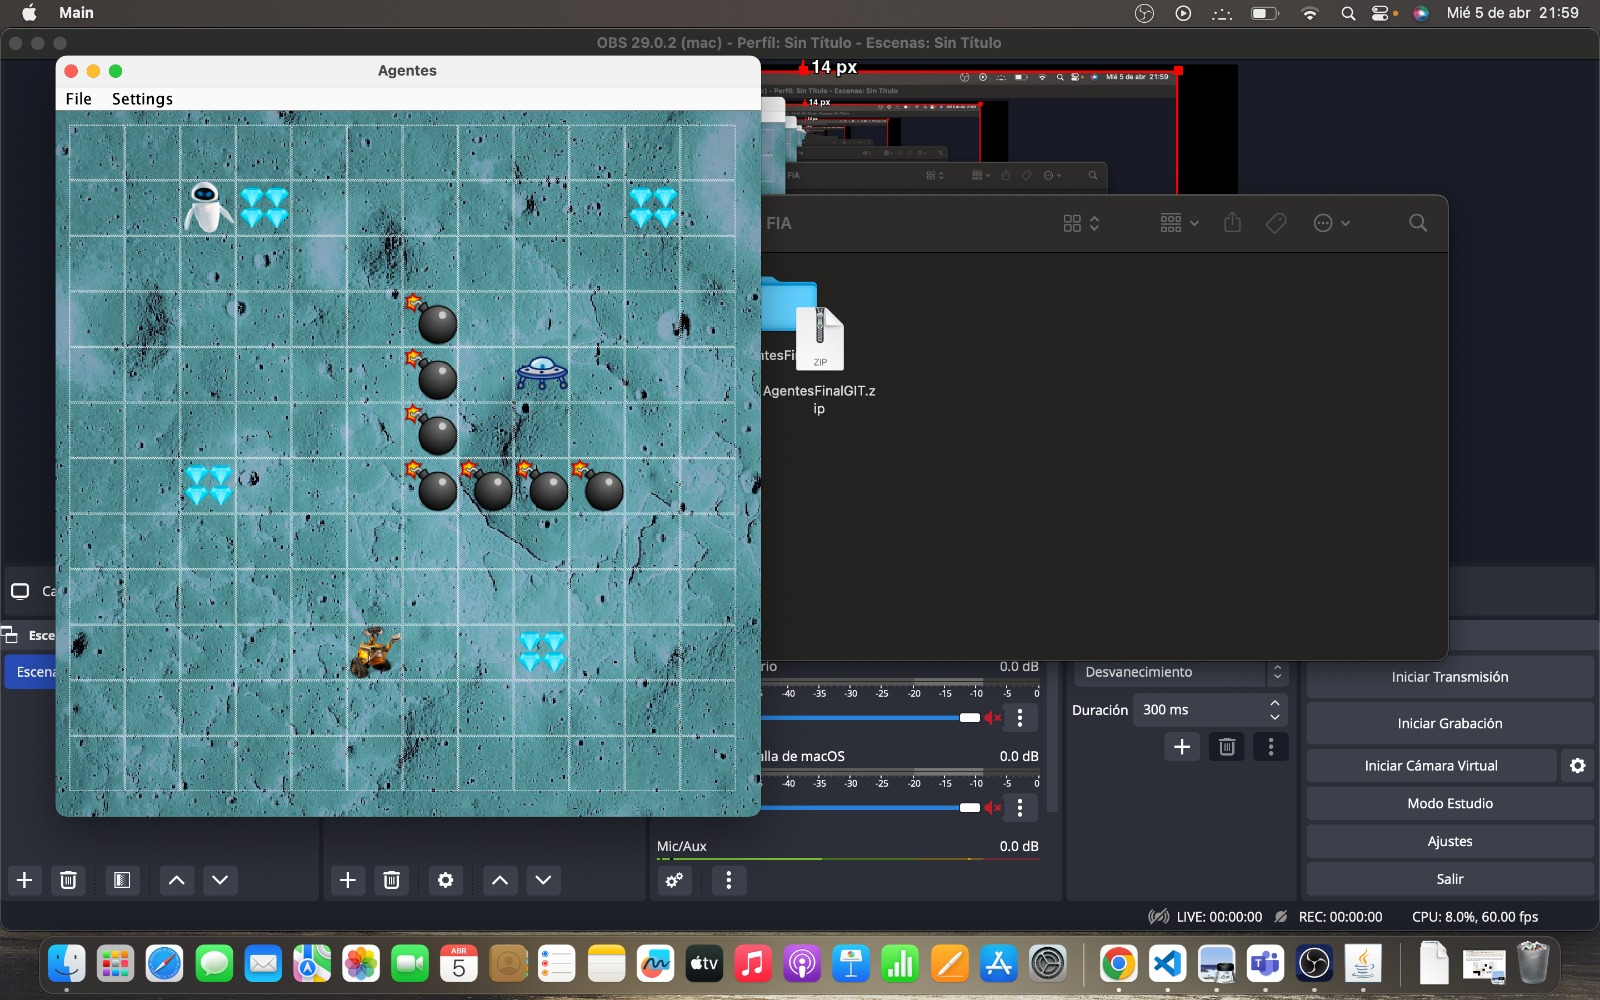
\includegraphics[scale=0.20]{demo.jpeg}\\
Este es el estado inicial del juego, colocamos los obstáculos y los clústeres de muestras.
A pesar de que los obstáculos estén bloqueando directamente a la nave, logran llegar a la nave, porque conocen el destino.

\includegraphics[scale=0.20]{demo2.jpeg}\\
Ahora hay migas, y los agentes dejan las \emph{muestras}, que en este caso son botes de basura para contaminar el mundo.

\includegraphics[scale=0.20]{demo3.jpeg}\\
\includegraphics[scale=0.20]{demo4.jpeg}\\
\includegraphics[scale=0.20]{demo5.jpeg}\\
Una demostración de cómo los robots siguen el rastro.

\section{Conclusiones}
En esta práctica se implementó el algoritmo A* para la búsqueda informada y se mejoró la funcionalidad de los agentes añadiendo un seguimiento de muestras. El objetivo principal del algoritmo A* es encontrar la ruta más corta entre un nodo de inicio y un nodo de destino en un grafo ponderado. Además, A* utiliza una heurística para estimar el costo restante del camino desde el nodo actual hasta el nodo objetivo, lo que le permite elegir la mejor opción de manera más efectiva que los algoritmos de búsqueda ciega. En esta práctica, la heurística utilizada por A* debe ser admisible, lo que significa que nunca debe sobreestimar el costo del camino restante. Se demostró que el algoritmo A* es un algoritmo óptimo y completo, lo que significa que siempre encuentra la ruta más corta si existe una y siempre termina si hay una solución.

Además, se implementó la funcionalidad de seguimiento de muestras, que permite a los agentes detectar si hay más muestras cerca de una muestra recolectada anteriormente. Esto mejora la eficiencia del agente al recolectar múltiples muestras a la vez en lugar de regresar a la nave espacial para cada muestra recolectada individualmente. Aunque fue complejo también determinar la dirección de movimiento de las muestras; pero nos permitió ver las ventajas y desventajas de los sistemas de comunicación indirecta.

Esta práctica fue exitosa en la implementación del algoritmo A* y la mejora de la funcionalidad de los agentes para una mayor eficiencia en la recolección de muestras. 
\end{document}